% This file was created with tikzplotlib v0.10.1.
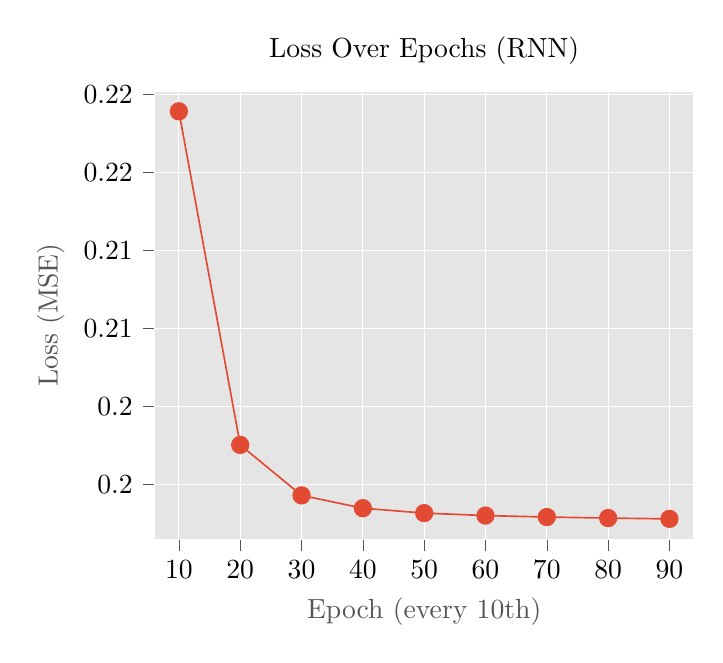
\begin{tikzpicture}

\definecolor{chocolate2267451}{RGB}{226,74,51}
\definecolor{dimgray85}{RGB}{85,85,85}
\definecolor{gainsboro229}{RGB}{229,229,229}

\begin{axis}[
axis background/.style={fill=gainsboro229},
axis line style={white},
tick align=outside,
tick pos=left,
title={Loss Over Epochs (RNN)},
x grid style={white},
xlabel=\textcolor{dimgray85}{Epoch (every 10th)},
xmajorgrids,
xmin=-0.4, xmax=8.4,
xtick style={color=dimgray85},
xtick={0,1,2,3,4,5,6,7,8},
xtick={0,1,2,3,4,5,6,7,8},
xticklabels={10,20,30,40,50,60,70,80,90},
xticklabels={10,20,30,40,50,60,70,80,90},
y grid style={white},
ylabel=\textcolor{dimgray85}{Loss (MSE)},
ymajorgrids,
ymin=0.191502721607685, ymax=0.220240204036236,
ytick style={color=dimgray85}
]
\addplot [semithick, chocolate2267451, mark=*, mark size=3, mark options={solid}]
table {%
0 0.218933954834938
1 0.197551742196083
2 0.194316670298576
3 0.193493545055389
4 0.193179294466972
5 0.193022191524506
6 0.192927539348602
7 0.19286160171032
8 0.192808970808983
};
\end{axis}

\end{tikzpicture}
